\section{Results}
\begin{frame}
    \sectionpage
\end{frame}

\begin{frame}{Execution time}
    \begin{figure}
        \centering
        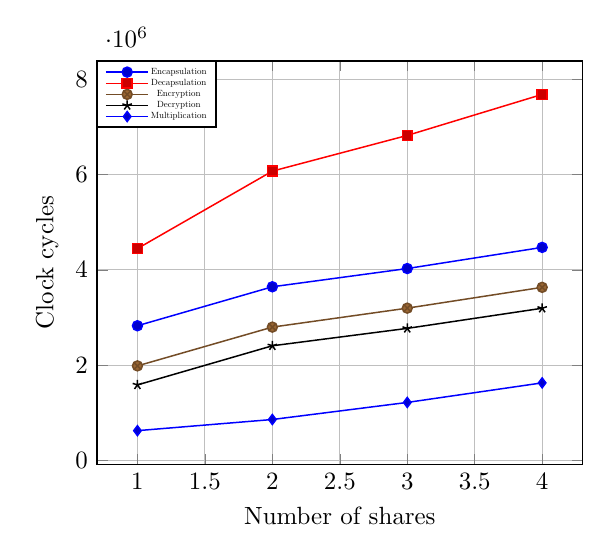
\begin{tikzpicture}[scale=0.9]
            \pgfplotsset{every axis/.append style={semithick}, legend style={at={(0,1)},anchor=north west, nodes={scale=0.6, transform shape}}}
    
        \begin{axis}[
            xlabel=Number of shares,ylabel=Clock cycles, grid=major,     x tick label style={
                /pgf/number format/.cd,
                precision=1,
            }]
    
        \addplot coordinates{
            (1, 2826067.47)
            (2, 3643555.40)
            (3, 4026514.86)
            (4, 4470225.81)
    
        };
        \addlegendentry{Encapsulation}
    
        \addplot coordinates{
            (1, 4445614.60)
            (2, 6070401.90)
            (3, 6819468.72)
            (4, 7680073.11)
    
        };
        \addlegendentry{Decapsulation}
    
        \addplot coordinates{
            (1, 1983894.79)
            (2, 2797433.27)
            (3, 3195107.26)
            (4, 3632298.13)
    
        };
        \addlegendentry{Encryption}
    
        \addplot coordinates{
            (1, 1584503.47)
            (2, 2405541.52)
            (3, 2770976.91)
            (4, 3193077.76)
    
        };
        \addlegendentry{Decryption}
    
        \addplot coordinates{
            (1, 624965.27)
            (2, 858842.66)
            (3, 1216993.20)
            (4, 1627512.25)
    
        };
        \addlegendentry{Multiplication}
        \end{axis}%
    \end{tikzpicture}%
    \end{figure}
\end{frame}

\begin{frame}{Execution Time}
    \begin{block}{Execution time (milliseconds)}
        \begin{table}
            \begin{tabular}{llllll}
                \# & encaps & decaps & enc & dec & mul \\ \hline
                1 & 201.86 & 317.54 & 141.71 & 113.18 & 44.64 \\
                2 & 260.25 & 433.60 & 199.82 & 171.82 & 61.35 \\
                3 & 287.61 & 487.10 & 228.22 & 197.93 & 86.93 \\
                4 & 319.30 & 548.58 & 259.45 & 228.08 & 116.25             
            \end{tabular}
        \end{table}
    \end{block}
    \begin{block}{Percentual performance decrease}
        \begin{table}
            \begin{tabular}{llllll}
                \# & encaps & decaps & enc & dec & mul \\ \hline
                2 & 28.92 & 36.55 & 41.00 & 51.81 & 37.42 \\
                3 & 42.48 & 53.40 & 61.05 & 74.88 & 94.73 \\
                4 & 58.18 & 72.76 & 83.09 & 101.51 & 160.41
            \end{tabular}
        \end{table}
    \end{block}
\end{frame}

\begin{frame}{Constant-time execution}
    \begin{block}{Welch's t-test}
        Given two statistical populations $X_1$ and $X_2$ of $N_1$ and $N_2$ samples respectively:
        \begin{equation*}
            t = \frac{\bar{X_1} - \bar{X_2}}{\sqrt{\frac{s_{X_1}^2}{N_1} + \frac{s_{X_2}^2}{N_2}}}
        \end{equation*}\\
    Can be used to verify that the means of the distributions are equal (null hypothesis).\\
    Setting the confidence to 99.999\%, we accept $H_0$ for $|t| \leq 4.5$
    \end{block}
\end{frame}

\begin{frame}{Constant-time execution}
    \begin{block}{Test Vector Leakage Assessment}
        Based on the Welch's t-test, defines the two groups as:
        \begin{itemize}
            \item Random: use different inputs for each computation
            \item Fixed: use the same inputs for all computations
        \end{itemize}
        In case of random data (\textit{e.g.} masks), these are always generated randomly.
    \end{block}
\end{frame}

\begin{frame}{Constant-time execution}
    \begin{block}{Welch's t}
        \begin{table}
            \begin{tabular}{llllll}
                \# & encaps & decaps & enc & dec & mul \\ \hline
                1 & 0.93666 & 4.56649 & 25.66178 & 10.26449 & 30.09420 \\
                2 & 6.00482 & 3.35650 & 4.62100 & 5.96089 & 4.96460 \\
                3 & 0.28901 & 1.69393 & 1.59911 & 5.88290 & 3.50812 \\
                4 & 0.12693 & NA\footnote{Not enough memory} & 3.30161 & 4.01299 & 0.21834
            \end{tabular}
        \end{table}        
    \end{block}
\end{frame}
